\documentclass[letterpaper]{article}

\usepackage{graphicx}  %Required
\usepackage{amsmath,amsfonts,amssymb}

\title{Supplementary Material:\\Disentangled Representation Learning for Non-Parallel Text Style Transfer}


\date{}
\author{}
\begin{document}
\maketitle
\graphicspath{{images/}}

\newcommand{\loss}[1]{J_{\text{#1}}}

These figures represent a few of the ablation tests in the form of t-SNE plots.

\begin{figure}[ht]
	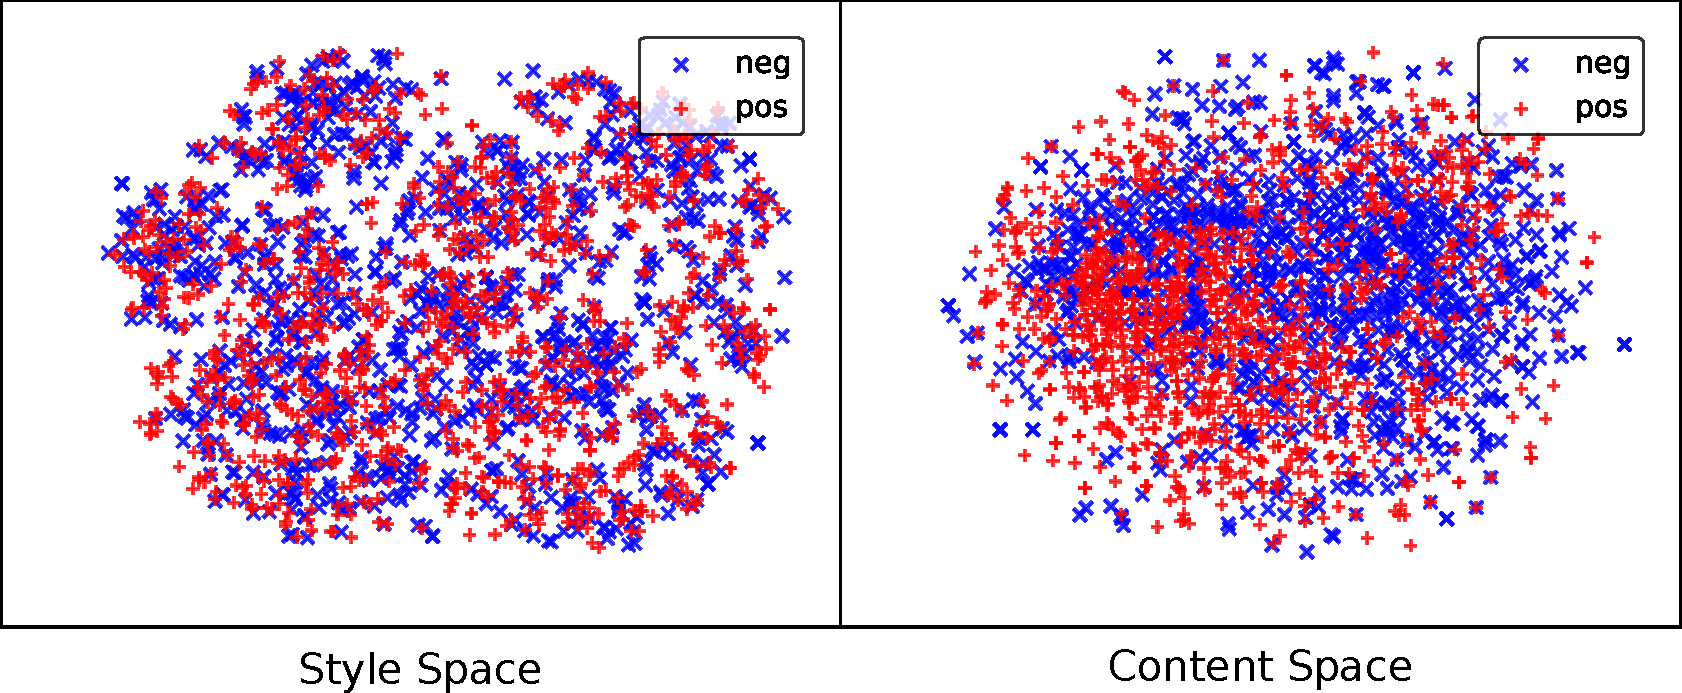
\includegraphics[width=\linewidth]{vae-latent-spaces-only-rec}
	\caption{t-SNE Plot of VAE latent embeddings with only $\loss{AE}$.}
\end{figure}

\begin{figure}[ht]
	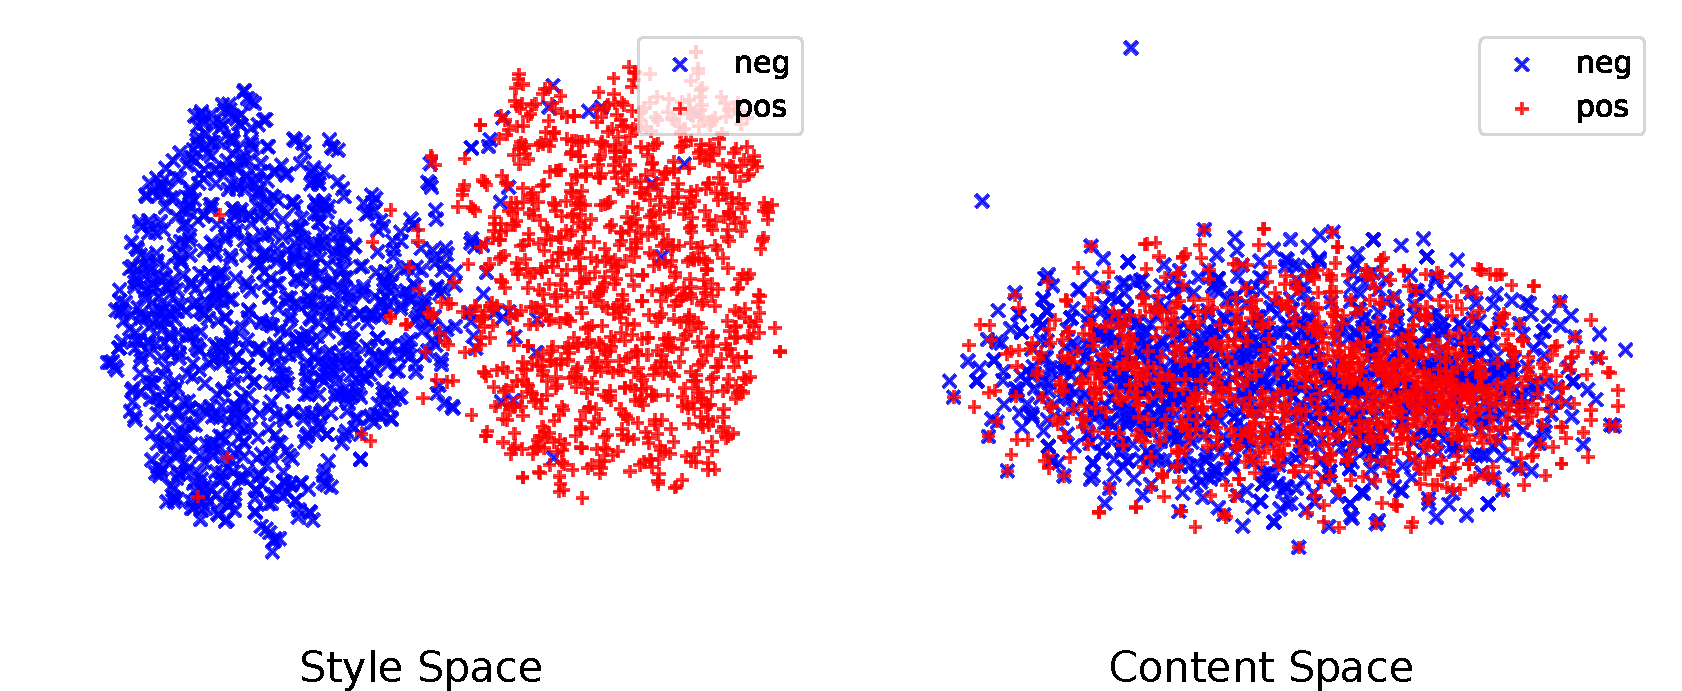
\includegraphics[width=\linewidth]{vae-latent-spaces-rec-muls}
	\caption{t-SNE Plot of VAE latent embeddings with $\loss{AE} + \loss{mul(s)}$.}
\end{figure}

\begin{figure}[ht]
	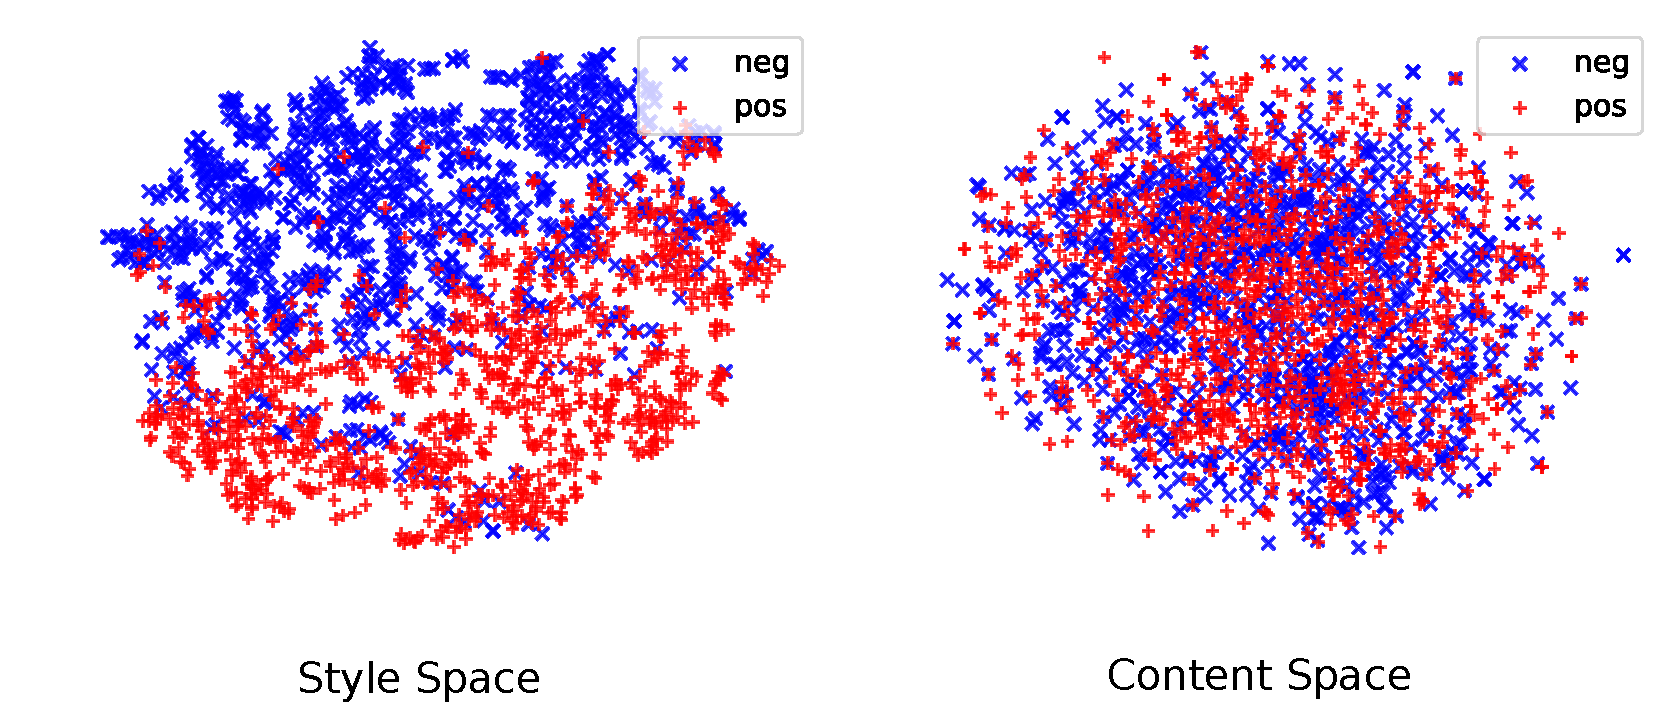
\includegraphics[width=\linewidth]{vae-latent-spaces-rec-advs}
	\caption{t-SNE Plot of VAE latent embeddings with $\loss{AE} + \loss{adv(s)}$.}
\end{figure}

\begin{figure}[ht]
	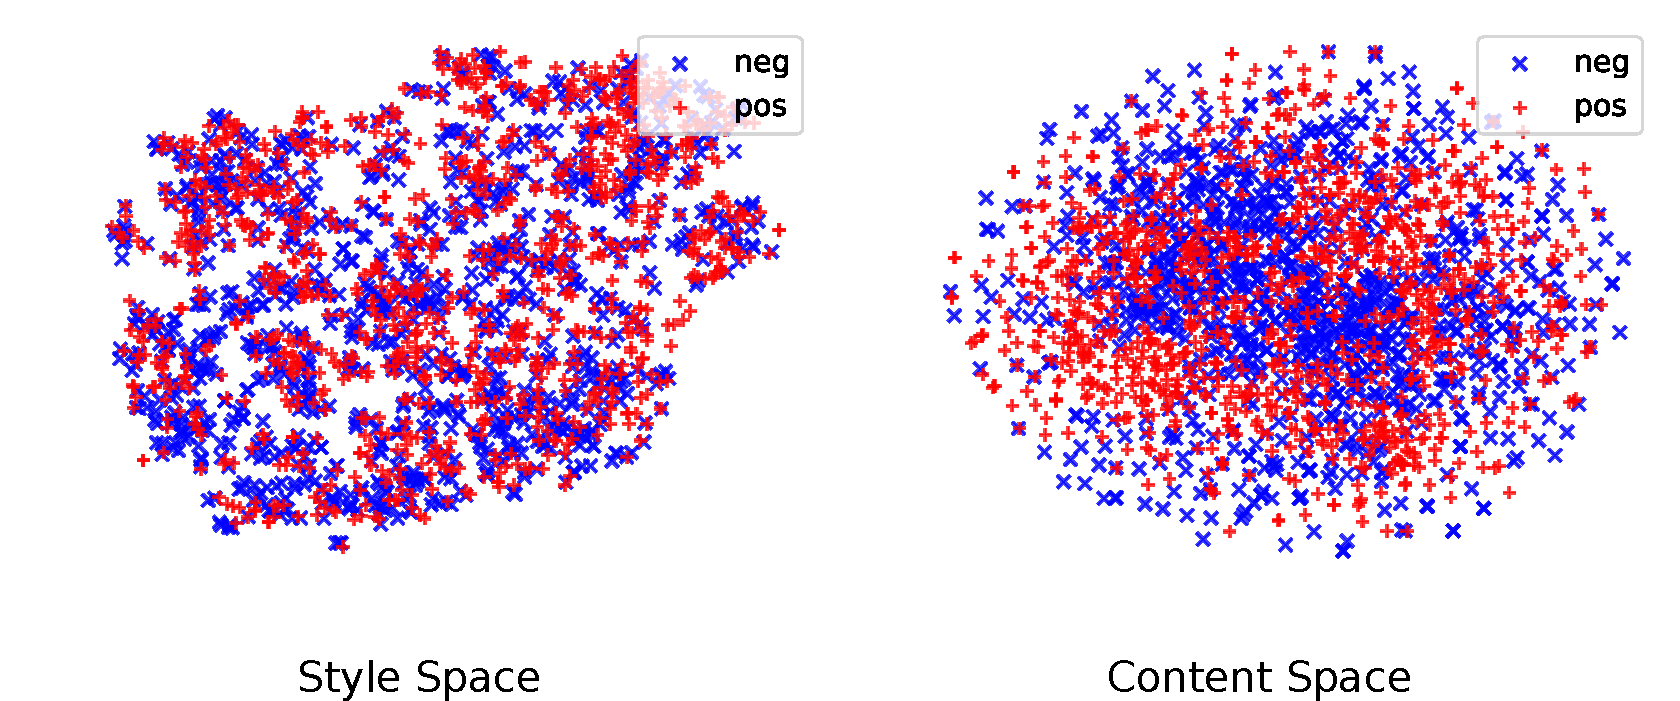
\includegraphics[width=\linewidth]{vae-latent-spaces-rec-mulc}
	\caption{t-SNE Plot of VAE latent embeddings with $\loss{AE} + \loss{mul(c)}$.}
\end{figure}


\begin{figure}[ht]
	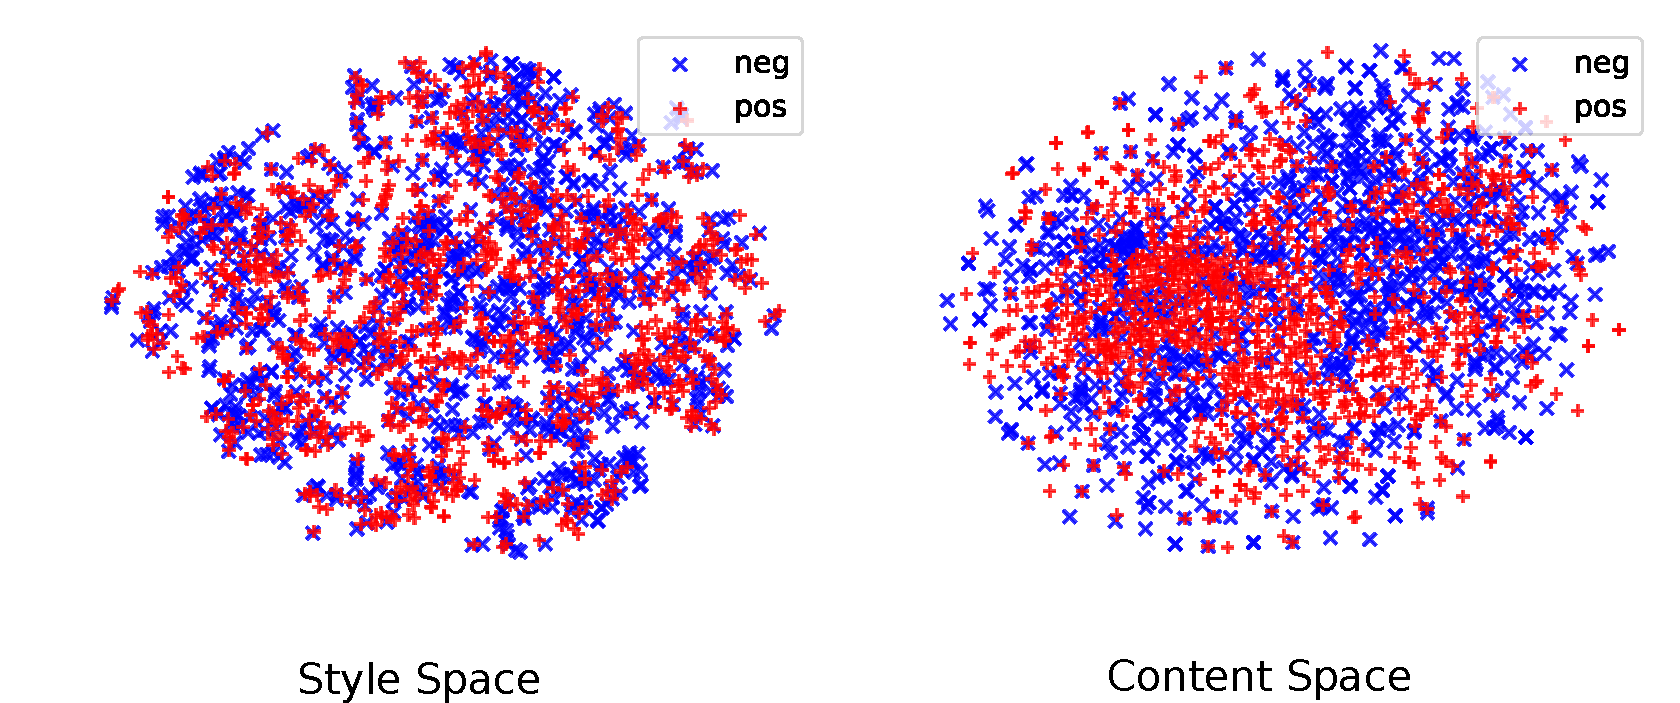
\includegraphics[width=\linewidth]{vae-latent-spaces-rec-advc}
	\caption{t-SNE Plot of VAE latent embeddings with $\loss{AE} + \loss{adv(c)}$.}
\end{figure}


\end{document}
